\documentclass[specialist,
               substylefile = spbu.rtx,
               subf,href,colorlinks=true, 12pt]{disser}

\usepackage[a4paper,
            mag=1000, includefoot,
            left=3cm, right=1.5cm, top=2cm, bottom=2cm, headsep=1cm, footskip=1cm]{geometry}
\usepackage[T2A]{fontenc}
\usepackage[utf8]{inputenc}
\usepackage[english,russian]{babel}
\ifpdf\usepackage{epstopdf}\fi


\usepackage{ucs}
\usepackage{cite}
\usepackage{amsmath}
\usepackage{amsthm}
\usepackage{amsfonts}
\usepackage{amssymb}
\usepackage{nicefrac}
\usepackage{csvsimple}
\usepackage[table,xcdraw]{xcolor}

\usepackage[linesnumbered,ruled]{algorithm2e}
\SetKwInput{KwData}{Исходные параметры}
\SetKwInput{KwResult}{Результат}
\SetKwInput{KwIn}{Входные данные}
\SetKwInput{KwOut}{Выходные данные}
\SetKwIF{If}{ElseIf}{Else}{если}{тогда}{иначе если}{иначе}{конец}
\SetKwFor{While}{пока}{выполнять}{конец}
\SetKw{KwTo}{от}
\SetKw{KwRet}{возвратить}
\SetKw{Return}{возвратить}
\SetKwBlock{Begin}{начало блока}{конец блока}
\SetKwSwitch{Switch}{Case}{Other}{Проверить значение}{и выполнить}{вариант}{в противном случае}{конец варианта}{конец проверки значений}
\SetKwFor{For}{цикл}{выполнять}{конец цикла}
\SetKwFor{ForEach}{для каждого}{выполнять}{конец цикла}
\SetKwRepeat{Repeat}{повторять}{до тех пор, пока}
\SetAlgorithmName{Алгоритм}{алгоритм}{Список алгоритмов}

\usepackage{graphicx}


% Использовать полужирное начертание для векторов
\let\vec=\mathbf

% Включать подсекции в оглавление
\setcounter{tocdepth}{2}

\graphicspath{{fig/}}


\theoremstyle{definition}
\newtheorem{definition}{Определение}

\newtheorem{theorem}{Теорема}
\newtheorem{lemma}{Лемма}

% Expectation symbol
\DeclareMathOperator*{\E}{\mathrm{E}}
\DeclareMathOperator*{\D}{\mathrm{D}}
\DeclareMathOperator*{\sign}{sign}
\DeclareMathOperator*{\argmin}{arg\,min}
\DeclareMathOperator*{\Int}{Int}
\DeclareMathOperator*{\err}{err}

\newcommand{\hm}[1]{#1\nobreak\discretionary{}{\hbox{\ensuremath{#1}}}{}}
\newcommand\norm[1]{\left\lVert#1\right\rVert}
\newcommand\abs[1]{\left\lvert#1\right\rvert}


%----------------------------------------------------------------
\begin{document}


\institution{%
    Санкт-Петербургский государственный университет
}

\title{Выпускная квалификационная работа}

% Тема
\topic{
    Оптимальные планы для оценивания производных в полиномиальной регрессионной модели без свободного члена}

% Автор
\author{Барсуков Егор Вячеславович}

\group{%
    Уровень образования: бакалавриат\\
    Направление 01.03.02 <<Прикладная математика и информатика>>\\
    Основная образовательная программа СВ.5004.2016 <<Прикладная математика и информатика>> \\
    Профиль <<Вычислительная стохастика и статистические модели>>
}

% Научный руководитель
\sa       {В.\,Б.~Мелас}
\sastatus {
Профессор кафедры статистического моделирования\,\\
д.\,ф.-м.\,н., профессор}

%Рецензент
\rev      {Ю.\,Д.~Григорьев}
\revstatus{Профессор кафедры математического обеспечения и применения ЭВМ, Санкт-Петербургский государственный электротехнический университет <<ЛЭТИ>> 
д.\,т.\,н., профессор}

% Город и год
\city{Санкт-Петербург}
\date{2020}

\maketitle


\tableofcontents

\addcontentsline{toc}{chapter}{Введение}
\chapter*{Введение}

  Рассмотрим регрессионную модель

  \begin{equation}
  \label{eq:regres}
    y_j = \theta^\top f(x_j) + \varepsilon_j, \quad j = 1 \ldots N, \, x_j \in \mathcal{X},
  \end{equation}
  где $N$ --- количество экспериментов, $\mathcal{X} \subset \mathbb{R}$, $f(x) = \left(f_1(x), \ldots, f_n(x) \right)^\top$ --- регрессионная функция, $\theta = \left( \theta_1, \ldots, \theta_n \right)^\top$ --- неизвестные параметры, $\varepsilon_i$ ---  некоррелированные ошибки наблюдения. При этом $\E [\varepsilon_i] = 0$, $\D [\varepsilon_i] = \sigma^2$.
  
  Для того, чтобы при фиксированном количестве наблюдений $N$ получить наилучшую в каком-либо смысле оценку $\theta$ строят \textit{планы эксперимента} т.е. наборы точек $x_i \in \mathcal{X}$, в каждой из которых должно быть произведено $n_i$ экспериментов так, что $\sum^N_i n_i = N$. В каком именно смысле будет улучшена оценка параметров модели зависит от выбора одного из нескольких критериев оптимальности.
  
  В работе будут рассматриваться полиномиальные регрессионные модели без нулевого члена, при этом регрессионная функция имеет вид $f(x) = (x, \ldots, x^n)^\top$. Для таких моделей во многих случаях явным образом были описаны оптимальные планы. Несколько работ были посвящены нахождению $\mathrm{D}$-оптимальных планов \cite{hoel1958, studden1980, dette1990, dette2001}. Также существуют для такой модели явные решения для нахождения $\mathrm{E}$-оптимальных планов \cite{pukelsheim1993, dette1993, heiligers1994, dette1993_2}.
  
  В этой работе будут рассматриваться $c$-оптимальные планы эксперимента. Ими называются планы, минимизирующие дисперсию значения скалярного произведения $\theta$ и $c$ для заданного $c \in \mathbb{R}^n$ \cite{dette1993_2}. В общем случае нахождение $c$-оптимальных планов может быть достаточно сложным: для случаев малой размерности решение можно найти используя теорему Элвинга \cite{elfving1952}, однако явного решения для произвольного $c$ не существует.
  
  В практических приложениях важны частные случаи: $c = f(z)$ для некоторого $z \notin \mathcal{X}$ --- задача экстраполяции в точке $z$ и $c = f'(z)$ --- задача оценки производной в точке $z$. Для обычной полиномиальной модели оптимальный план экстраполяции был получен достаточно давно \cite{hoel1964}, также существует несколько явных решений для задачи оценки производной в некоторых случаях \cite{melas2010, melasmain}.
  
  В этой работе рассмотрен случай нахождения планов для оценки производной при полиномиальной модели без свободного члена при $\mathcal{X} = [0, d]$. Такая модель, например, может быть использована в тех случаях, когда, исходя из практической задачи, $z$ может принимать только положительные значения и существует априорное знание о значении функции в точке 0. Простым примером такой функции является зависимость расстояния от начальной точки от времени.
  
  Также в главе \ref{ch:num} построен алгоритм нахождения $c$-оптимальных планов в общем случае, который будет работать и для произвольных $c$ и для произвольных регрессионных функций, что позволяет применять $c$-оптимальные планы в различных практических задачах, для которых аналитические результаты либо недоступны, либо трудно применимы.

  
  
  

\chapter{C-оптимальные планы эксперимента}

\section{Определения}

  \begin{definition}
  Согласно \cite{kiefer1974} непрерывным планом эксперимента в регрессионной модели \eqref{eq:regres} будем называть дискретную вероятностную меру
  \begin{equation*}
    \xi = 
      \begin{pmatrix}
        x_1 & \ldots & x_m \\
        \omega_1 & \ldots & \omega_m
      \end{pmatrix}, \quad x_i \in \mathcal{X},
  \end{equation*}
   где $\omega_i \geqslant 0, \, \sum_i^n \omega_i = 1$, $i = 1, \ldots, m$.
  \end{definition}

  Для проведения $N$ измерений с мерой $\xi$ необходимо провести $n_i \approx N \omega_i$ измерений в точке $x_i$ таким образом, чтобы $\sum^m_i n_i = N$.

  \begin{definition}
  Информационной матрицей для непрерывного плана эксперимента, заданного мерой $\xi$, является 
  \begin{equation*}
    M(\xi) = \int_{\mathcal{X}} f(x) f^\top(x) \xi (dt).
  \end{equation*}
  \end{definition}
  
  \begin{definition}
  \label{def:coptim}
  \textit{$c$-оптимальным планом} для некоторого вектора $c$ называется план эксперимента $\xi$, минимизирующий функцию
  \begin{equation}
  \label{eq:cdef}
    \Phi(\xi) = \begin{cases}
      c^\top M(\xi)^{-} c, \quad \text{если существует } v \text{, такой, что } \; c = M(\xi) v\\
      +\infty, \quad  \text{иначе}
    \end{cases},
  \end{equation}
  где $M(\xi)^{-}$ --- обобщенно обратная матрица к информационной матрице плана $\xi$.
  План называется допустимым, если существует такой $v$, что $c = M(\xi) v$.
  \end{definition}
  
  Как было отмечено во введении, $c$-оптимальный план минимизирует дисперсию несмещенной оценки по методу наименьших квадратов $c^\top \hat{\theta}$ линейной комбинации $c^\top \theta$~\cite{dette1993_2}.
 
  \begin{definition}
  Если $c = f'(z)$ для некоторого $z \in \mathbb{R}$, то соответствующий $c$-оп\-ти\-маль\-ный план называется \textit{оптимальным планом для оценки производной} в точке $z$.
  \end{definition}
  
  \section{Теорема Элвинга}
  
  Для решения задачи нахождения $c$-оптимальных планов во множестве случаев (в том числе в данной работе) используется теорема Элвинга, являющаяся критерием $c$-оптимальности плана эксперимента.
  \begin{theorem}
  \label{th:elfving}
  (Элвинга) \cite{melas2010}
  Допустимый план $\xi^\star$ с носителем $x_1, \ldots, x_m \in \mathcal{X}$ и весами $\omega_1, \ldots, \omega_m$ является $c$-оптимальным тогда и только тогда, когда существует $p \in \mathbb{R}^n$ и константа $h$ такие, что выполняются следующие условия:
  \begin{subequations}
  \label{eq:elfving}
  \begin{align}
	&\abs{p^\top f(x_i)} = 1, &&i=1..m \leqslant n \label{eq:elfving:eq1} ,\\
	&\abs{p^\top f(x)} \leqslant 1,  &&x \in \mathcal{X} \label{eq:elfving:eq2} ,\\
	&c = h \sum_{i=1}^m \omega_i f(x_i) p^\top f(x_i) \label{eq:elfving:eq3}.
  \end{align}
  Кроме того
  \begin{equation*}
  	h^2 = c^\top M^{-}(\xi^{*})c.
  \end{equation*}
  \end{subequations}
  \end{theorem}
	Функция $p^\top f(x)$ в обозначениях теоремы Элвинга в этой работе также будет называться \textit{экстремальным многочленом}.
	
	\section{Явная формула для весов оптимального плана}
	
	\begin{theorem} \cite{melasmain}
	\label{th:weights}
	Оптимальный план для оценивания производной полиномиальной модели без свободного члена с опорными точками $t_1^*, \ldots, t_m^*$, где $m=n$ или $m=n-1$ имеет веса, вычисленные по следующей формуле:	
	
	\begin{equation}
	\label{eq:weights}
		\omega_i = \frac{\abs{L'_i(z)}}{\sum_{j=1}^m \abs{L'_j(z)}},
	\end{equation}
	где $L_i$ задается следующим образом
	\begin{equation}
		\label{eq:lagr}
		L_{i}(x) = \frac{x \prod_{l \neq i} (x - t_l^*)}{t_i^* \prod_{l \neq i} (t_i^* - t_l^*)},
	\end{equation}	
	то есть является многочленом без нулевого члена степени $m$, который равен 1 в точке $t_i^*$ и нулю в остальных опорных точках. Такой многочлен далее в этой работе будет называться $i$-ым базисным многочленом Лагранжа без нулевого члена построенным по точкам $t_1^*, \ldots, t_m^*$.
	\end{theorem}
	
	
	
  
	\chapter{Оптимальный план на отрезке с началом в нуле для оценки производной}
  
  В этой главе описаны оптимальные планы на отрезке $[0, d]$ для оценки производной в модели без нулевого члена. Как было отмечено ранее, необходимость в таких планах может возникать в некоторых практических задачах. С точки зрения решения эта задача отличается от случая носителя $[-1, 1]$, которая была рассмотрена в \cite{melasmain}, тем, что экстремальный многочлен должен обладать другими свойствами. В разделе \ref{sec:01}  рассмотрен случай отрезка $[0,1]$, а в разделе \ref{sec:0d} рассмотрены отличия для промежутка общего вида $[0, d]$, в конце главы приведен пример применения доказанной теоремы.
  
  Везде в этой главе считается, что $f(x) = (x, x^2, \ldots, x^n)^\top$, то есть рассматривается модель без нулевого члена.
  
  \section{Промежуток [0, 1]}
  \label{sec:01}
  
  При доказательстве основной теоремы этой главы будет использована следующая лемма.
  
  \begin{lemma}
  \label{lemma:droots}
  	Пусть $P_1(x)$ и $P_2(x)$ --- многочлены степени $n$ с корнями $t^1_1 < \ldots < t^1_n$ и $t^2_1 < \ldots < t^2_n$ соответственно. При этом корни располагаются следующим образом:
  	\begin{equation*}
  		t^1_1 \leqslant t^2_1 \leqslant t^1_2 \leqslant t^2_2 \leqslant \ldots \leqslant t^1_n \leqslant t^2_n,
  	\end{equation*}
  	где хотя бы одно из неравенств $t_l^1 \leqslant t_l^2$ ($l = 1, \ldots, n$) является строгим. Также обозначим корни многочленов $P'_1(x)$ и $P'_2(x)$ как $v_1^1, \ldots, v_{n-1}^1$ и $v_1^2, \ldots, v_{n-1}^2$. Тогда справедливо следующее утверждение
  	\begin{equation*}
  		v^1_1 < v^2_1 < v^1_2 < v^2_2 < \ldots < v^1_{n-1} < v^2_{n-1}.
  	\end{equation*}
  \end{lemma}
  Доказательство этого утверждения можно найти в \cite{sahmphd} или в приложении к \cite{melasmain}.
  
  Следующая лемма дает вид экстремального многочлена, необходимого для проверки критерия $c$-оптимальности для промежутка $[0, 1]$ в полиномиальной модели без нулевого члена.
  
  \begin{lemma}
  \label{lemma:extrpoly}
  Пусть $T_n(x)$ --- многочлен Чебышева первого рода степени $n$. Тогда 
  	\begin{equation}
  	\label{eq:extrpoly}
  		S_n(x) = T_n \left(x \left(1 + \cos \frac{\pi}{2n} \right) - \cos \frac{\pi}{2n} \right)
	\end{equation}   
	является многочленом степени $n$ без нулевого члена, который на промежутке $[0, 1]$ не превосходит по модулю единицу, при этом равенство достигается ровно в $n$ точках $x^*_i$:
	\begin{equation}
	\label{eq:extrpolyroots}
		x_i^* = \frac{\cos \frac{(n - i) \pi}{n} + \cos \frac{\pi}{2n}}{1 + \cos \frac{\pi}{2n}} , \, i = 1, \ldots n.
	\end{equation}
  \end{lemma}
  
  \begin{proof}
  	Известно, что многочлены Чебышева первого рода не превосходят по модулю единицу на отрезке $[-1, 1]$ и при этом равенство достигается в $n+1$ точках. По построению $S_n(x)$ удовлетворяет этим же свойствам, но на отрезке $[-\cos \frac{\pi}{2 n}, 1]$. Так как $-\cos \frac{\pi}{2 n}$ --- наименьший корень $T_n(x)$, и он больше всего одной его точки экстремума $\tilde{x}_0^*\hm{=}-1$, то $S_n(x)$ --- многочлен без нулевого члена, не превосходящий по модулю единицу на промежутке $[0, 1]$ и достигающий ее ровно $n$ раз. Из известных экстремальных точек многочленов Чебышева и построения $S_n(x)$ следует, что его равенство единице по модулю достигается в \eqref{eq:extrpolyroots}.
  \end{proof}
  
  Следующая теорема формулирует условия, когда многочлен \eqref{eq:extrpoly} действительно определяет план для оценки производной. 
	
	\begin{theorem}
	\label{th1}
		Пусть для $i = 1, \ldots, n$ корни производной многочлена $L_i$ из~\eqref{eq:lagr}, построенного по точкам \eqref{eq:extrpolyroots}, равны $u_1^i, \ldots, u_{n-1}^i$, причем $u_k^i < u_l^i$ при $k < l$. Тогда план с опорными точками \eqref{eq:extrpolyroots} и весами \eqref{eq:weights} является оптимальным планом для оценки производной в точке $z$ в полиномиальной модели степени $n$ без свободного члена на промежутке $[0, 1]$, если выполнено одно из следующих условий:
		\begin{itemize}
			\item $z \in (-\infty, u_1^n)$,
			\item $z \in (u_{n-1}^1, +\infty )$,
			\item $z \in \left( u^1_j, u^n_{j+1} \right)$ для $j=1, \ldots, n-2$.
		\end{itemize}
	\end{theorem}
	\begin{proof}
		Доказательство теоремы сводится к проверке условий теоремы Элвинга. Выполнение условий \eqref{eq:elfving:eq1} и \eqref{eq:elfving:eq2} следует из леммы \ref{lemma:extrpoly}, если за $p$ взять вектор коэффициентов многочлена $S_n$. Поэтому для доказательства теоремы достаточно проверки условия \eqref{eq:elfving:eq3} при $c = f'(z)$.
	
	Так как теорема \ref{th:weights} о весах оптимального плана для оценки производной в случае полиномиальной модели выполняется для любых промежутков, то веса имеют вид \eqref{eq:weights}.
	
	Введем обозначения $F = \left((x_j^*)^i\right)^n_{i, j = 1}$ и $\beta = \left( \omega_i (-1)^{i+n} \right)_{i=1}^n$. Так как $x_j^*$ при $i\hm{=}1, \ldots , n$ являются экстремальными точками многочлена $S_n$ и при этом $S_n(x_j^*) = (-1)^{j+n}$, то выполнение равенства для некоторого $h$
	\begin{equation}
		\label{th:mateq3}
		f'(z) = hF\beta
	\end{equation}
	 эквивалентно выполнению условия \eqref{eq:elfving:eq3} теоремы Элвинга для нахождения оптимального плана оценки производной в точке $z$.
	 
	Утверждение $F^{-1}F = I_n$, где $I_n$ --- единичная матрица размера $n$, в силу того, что $i$--ый столбец матрицы $F$ на самом деле равен $f(x_i^*)$ ($i = 1, \ldots, n$), можно переписать, как систему равенств
	\begin{equation}
	\label{eq:deltas}
		e_i^{\top} F^{-1} f(x_j^*) = \delta_{ij} \, , \quad i, j = 1, \ldots , n ,
	\end{equation}
	где $\delta_{ij}$ --- дельта Кронекера, а $e_i$ --- $i$--ый единичный вектор. Поскольку в левой части \eqref{eq:deltas} содержатся многочлены без нулевого коэффициента степени не больше $n$, вычисленные в точках $x_j^*$, $j=1, \ldots , n$, а для каждого $i$ существует только одно $j$, такое, что $\delta_{ij} \neq 0$, то они определяют все базисные многочлены Лагранжа без нулевого члена степени $n$ вычисленные в точках $x_j^*$, $j=1, \ldots , n$, таким образом
	\begin{equation*}
		e_i^{\top} F^{-1} f(z) = L_i(z) \, , \quad i, j = 1, \ldots , n .
	\end{equation*}
	Если в предыдущем выражении вычислить производную по $z$, переписать полученное выражение в векторной форме и домножить обе части равенства слева на $F$ получим
	\begin{equation}
		\label{eq:vecleg}
		f'(z) = F \left( L'_1(z), \ldots, L'_n(z) \right)^\top.
	\end{equation}
	Приравняв правые части~\eqref{eq:vecleg} и~\eqref{th:mateq3} и домножив обе части равенства на $F^{-1}$ слева, получаем, что
	\begin{equation*}
		h \beta = \left( L'_1(z), \ldots, L'_n(z) \right)^\top,
	\end{equation*}
	что с учетом известного вектора $\beta$ и положив $h = \sum_{i=1}^n \abs{L'_i(z)}$ эквивалентно тому, что $\sign (L'_i(z)) = \sign((-1)^{i+n}) $, $i = 1, \ldots, n$ или, так как экстремальным многочленом также может быть $-S(x)$,  $\sign (L'_i(z)) = \sign((-1)^{i+n+1}) $, $i = 1, \ldots, n$.
	
	Таким образом для того, чтобы доказать, что оптимальный план находится в точках $(x_i^*)_{i=1}^n$ , $i = 1, \ldots, n$ с указными весами, осталось доказать равенство (или противоположность) знаков $L'_i(z)$ и $ S_n(x_i^*)$ для $i = 1, \ldots n$. Но так как знаки значений многочлена $S_n$ в экстремальных точках чередуются, достаточно проверить при каких $z$ выражения $(-1)^i L'_i(z)$ имеет одинаковый знак.
	
	Так как корни многочленов $L_i$ и $L_j$ для любых $i$ и $j$ таких, что $i < j$ удовлетворяют условию леммы \ref{lemma:droots}, то, последовательно её применяя ко всем базисным многочленам, получаем, что корни их производных, обозначения для которых были описаны в условии этой теоремы, удовлетворяют следующему соотношению:
	\begin{equation*}
		u^n_1 < u^{n-1}_1 < \ldots < u^1_1 < u^n_2 < u^{n-1}_2 < \ldots < u_{n-1}^1.
	\end{equation*}
	
	Так как все узловые точки больше нуля, знак многочлена $L_i(z)$ при $z \to -\infty$ будет равен $(-1)^{n+i+1}$. В то же время знак $L'_i(z)$ будет противоположным $L_i(z)$, так как меняется четность многочлена и при этом не меняется знак при старшем коэффициенте, то есть $\sign(L'_i(z)) = \sign((-1)^{n+i})$ при $z \to -\infty$. И, следовательно, $\sign((-1)^i L'_i(z)) = \sign((-1)^{n+2i}) = \sign((-1)^{n})$ при достаточно малом  $z $, то есть $\sign((-1)^i L'_i(z))$  имеет постоянный знак для любых $i$, что означает, что при $z \in (-\infty, u_1^n)$ третье условие теоремы Элвинга выполняется и план является оптимальным.
	
	На промежутках $[u_j^n, u_j^1]$ ($j = 1, \ldots {n-1}$) каждый базисный многочлен меняет свой знак ровно один раз и на этих промежутках знаки производных не совпадают со знаками экстремального многочлена, а на промежутках $(u_j^1, u_{j+1}^n)$ ($j=1, \ldots n-2$) нет ни одного корня и поэтому $\sign((-1)^i L'_i(z)) = \sign ((-1)^{n + j})$ при $z \in (u_j^1, u_{j+1}^n)$ ($j=1, \ldots n-2$), это подтверждает третье условие теоремы Элвинга в этих промежутках и показывает, что рассматриваемый план оптимален.
	
	На промежутке $(-\infty, u_{n-1}^1]$ каждый базисный многочлен поменял свой знак одинаковое количество раз, а так как при $z \to -\infty$ условие выполнялось, то при $z \in (u_{n-1}^1, +\infty)$ план также является оптимальным.
	
	Таким образом план эксперимента с опорными точками \eqref{eq:extrpolyroots} и соответствующими им весами \eqref{eq:weights} является оптимальным планом для оценки производной в точке $z$ в модели без нулевого члена тогда и только тогда, когда $z \in  (-\infty, u_1^n) \cup (u_{n-1}^1, +\infty)$ или $z \in (u_{j}^1, u_{j+1}^n)$ для $j=1, \ldots n-2$.

	\end{proof}
	
	\section{Произвольный промежуток с началом в нуле}
	\label{sec:0d}
	
	В общем случае полученные условия оптимальности для всех положительных промежутков, начинающихся в нуле, существенно не отличается от единичного отрезка. Пусть требуется найти условия оптимальности плана на промежутке $[0, d]$. Возьмем многочлен $S_n^d(x) = S_n(\frac{x}{d})$, пусть $\widehat{x_i^*}$ --- его экстремальные точки. Тогда
	\begin{equation}
	\label{eq:coorectedextr}
		\widehat{x_i^*} = d x_i^*, \, i = 1, \ldots, n
	\end{equation}
	где $x_i^*$ --- экстремальные точки $S_n$ из \eqref{eq:extrpolyroots}. $S_n^d(x)$ по построению по модулю не превышает единицу на промежутке $[0, d]$ и достигает единицы ровно $n$ раз, что необходимо для выполнения первых двух условий теоремы Элвинга. Построив базисные многочлены по точкам \eqref{eq:coorectedextr} вместо \eqref{eq:extrpolyroots} условия и дальнейшее доказательство теоремы \ref{th1} полностью переносятся на случай промежутка $[0, d]$.
	
	
	\section{Пример для полиномиальной модели третьей степени}
	\label{sec:ex}
	С помощью доказанной теоремы найдем некоторые планы для оценки производной в модели $f(x)  = (x, x^2, x^3)^\top$ с областью планирования $\mathcal{X} = [0, 1]$. Экстремальный многочлен согласно \eqref{eq:extrpoly} в этом случае равен 
	\begin{align*}
		S_3(x) &= T_3\left(x \left(1 + \frac{\sqrt{3}}{2} \right) -  \frac{\sqrt{3}}{2} \right) \\ 
		&= \left(\frac{\sqrt{3}}{2}+1\right)^3 x^3-6 \sqrt{3} \left(\frac{\sqrt{3}}{2}+1\right)^2 x^2+6 \left(\frac{\sqrt{3}}{2}+1\right) x,
	\end{align*}
	\begin{figure}
		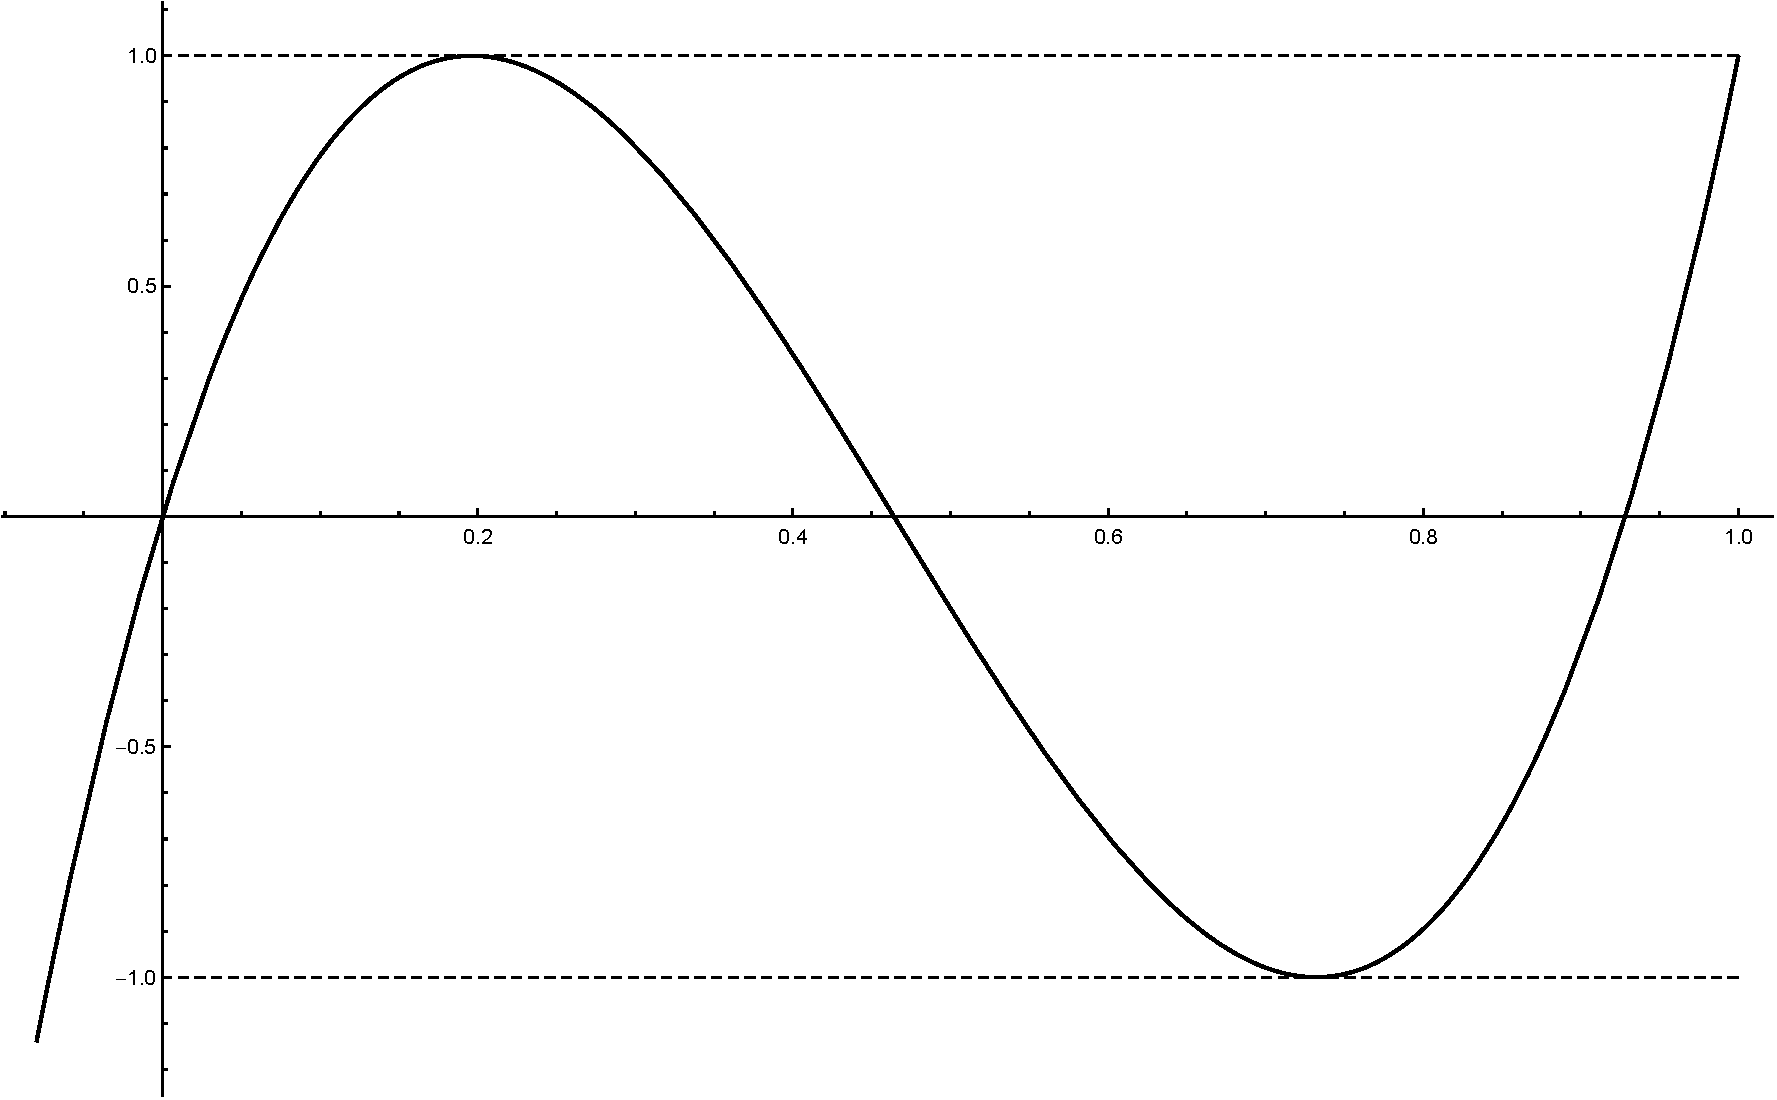
\includegraphics[width=\textwidth]{fig/s3.pdf}
		\caption{Экстремальный многочлен для $n = 3$.}
	\end{figure}
	а его экстремальные точки по \eqref{eq:extrpolyroots} равны 
	\begin{equation}
	\label{eq:ex:point}
		x_1^* = 3 \sqrt{3} - 5, \approx 0.1962 \quad x_2^* = \sqrt{3} - 1 \approx 0.7362, \quad x_3^* = 1.
	\end{equation}
	Тогда базисные многочлены \eqref{eq:lagr}, построенные по $x_1^*, \,x_2^*, \,x_3^*,$  выглядят следующим образом:
	\begin{align*}
		L_1(x) &= \frac{x (x - 1) (x - \sqrt{3} + 1)}{6 (41 \sqrt{3} - 71)}, \\
		L_2(x) &= \frac{x (x - 1) \left(x-3 \sqrt{3}+5\right)}{38 - 22 \sqrt{3}},\\
		L_3(x) &= \frac{1}{3} x \left(\left(4 \sqrt{3}+7\right) x^2-2 \left(2 \sqrt{3}+3\right) x+2\right) ,
	\end{align*}
	и, соответственно, их производные:
	\begin{align*}
		L'_1(x) &= \frac{3 x^2-2 \sqrt{3} x+\sqrt{3}-1}{6 \left(41 \sqrt{3}-71\right)}, \\
		L'_2(x) &= \frac{-3 x^2+\left(6 \sqrt{3}-8\right) x-3 \sqrt{3}+5}{22 \sqrt{3}-38}, \\
		L'_3(x) &= \left(4 \sqrt{3}+7\right) x^2+\left(-4-\frac{8}{\sqrt{3}}\right) x+\frac{2}{3}.
	\end{align*}
	Из производных базисных многочленов по \eqref{eq:weights} можно вычислить веса плана. Поскольку из доказательства теоремы известно, что на промежутках, где выполняется условие теоремы, знаки производных базисных многочленов чередуются, то для более простого явного вида формулу для весов можно переписать как
	\begin{equation*}
		\omega_i = \abs{\frac{L'_i(z)}{\sum_{j=1}^m (-1)^j L'_j(z)}}.
	\end{equation*}
	С учетом этого, веса можно явно выписать:
	\begin{align}
	\label{eq:ex:w}
	\begin{split}
		\omega_1 &= \frac{1}{12} \left(41 \sqrt{3}+71\right) \left| \frac{3 z^2-2 \sqrt{3} z+\sqrt{3}-1}{\frac{3}{2} z \left(14 \sqrt{3}-\left(15 \sqrt{3}+26\right) z+24\right)-3 \left(\sqrt{3}+2\right)}\right|, \\
		\omega_2 &=  \frac{1}{4} \left(11 \sqrt{3}+19\right) \left| \frac{z \left(-3 z+6 \sqrt{3}-8\right)-3 \sqrt{3}+5}{\frac{3}{2} z \left(14 \sqrt{3}-\left(15 \sqrt{3}+26\right) z+24\right)-3 \left(\sqrt{3}+2\right)}\right|, \\
		\omega_3 &= \left| \frac{z \left(\left(4 \sqrt{3}+7\right) z-\frac{8}{\sqrt{3}}-4\right)+\frac{2}{3}}{\frac{3}{2} z \left(-\left(15 \sqrt{3}+26\right) z+14 \sqrt{3}+24\right)-3 \left(\sqrt{3}+2\right)}\right|.
	\end{split}
	\end{align}
	
	Теперь осталось показать, при каких $z$ план с опорными точками \eqref{eq:ex:point} и весами \eqref{eq:ex:w} является оптимальным планов для оценки производной в точке $z$. Для этого найдем корни производных базисных многочленов (здесь для них используются обозначения из теоремы).
	\begin{align*}
		&u_1^1 = \frac{1}{3} \left(\sqrt{3}-\sqrt{3 \left(2-\sqrt{3}\right)}\right), &&u_2^1 = \frac{1}{3} \left(\sqrt{3}+\sqrt{3 \left(2-\sqrt{3}\right)}\right),\\
		&u_1^2 = \frac{1}{3} \left(3 \sqrt{3}-\sqrt{58-33 \sqrt{3}}-4\right), &&u_2^2 = \frac{1}{3} \left(3 \sqrt{3}+\sqrt{58-33 \sqrt{3}}-4\right), \\
		&u_1^3 = \frac{1}{3} \left(4 \sqrt{3}-\sqrt{2 \left(21-12 \sqrt{3}\right)}-6\right), &&u_2^3 = \frac{1}{3} \left(4 \sqrt{3}+\sqrt{2 \left(21-12 \sqrt{3}\right)}-6\right).\\
	\end{align*}
	Их приближенные значения:
	\begin{align*}
		&u_1^1 \approx 0.2784, &&u_2^1  \approx 0.8762,\\
		&u_1^2 \approx 0.0927, &&u_2^2 \approx 0.7046, \\
		&u_1^3 \approx 0.0906, &&u_2^3 \approx 0.5281.\\
	\end{align*}
	
	По теореме \ref{th1} план с опорными точками \eqref{eq:ex:point} и весами \eqref{eq:ex:w} является оптимальным планом для оценки производной если $z < u_1^3$, $z > u_2^1$ или $u_1^1 < z < u_2^3$.
	
	\begin{figure}
		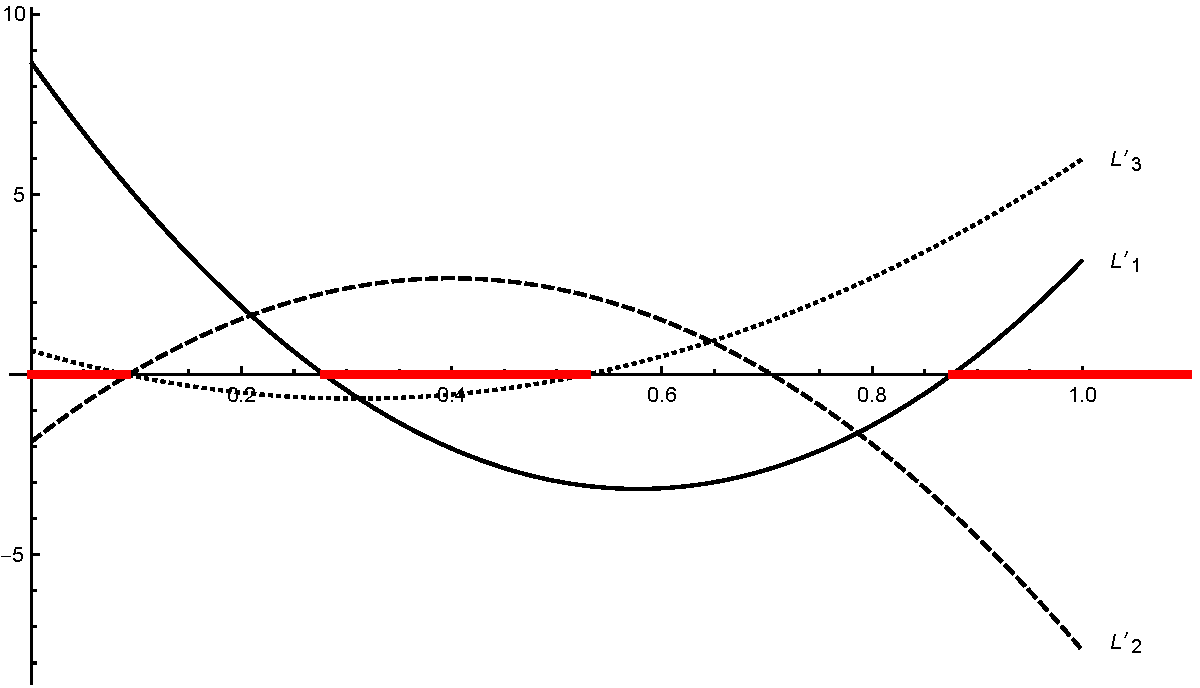
\includegraphics[width=\textwidth]{fig/dl_color.pdf}
		\caption{Производные базисных многочленов. Красным выделены промежутки, на которых выполняется теорема.}
	\end{figure}
	
	
\chapter{Численное нахождение с-оптимальных планов}
\label{ch:num}
	Как было показано в предыдущей главе, задача нахождения $c$-оптимальных планов далеко не всегда является тривиальной. Для многих случаев нет явных аналитических решений, а, даже там, где они существуют, не всегда просто их применять. В этой главе описан алгоритм численного нахождения и проверки $c$-оптимальных планов для произвольного $c$, работающий для модели общего вида.
	\section{Описание алгоритма}
	Пусть стоит задача построить $c$-оптимальный план для некоторого вектора $c$, в модели, заданной вектор-функцией $f(x) = (f_1, \ldots, f_n)^\top$, и область планирования $\mathcal{X} \hm{=} [a, b]$ является конечным отрезком.
	
	Определение $c$-оптимального плана уже содержит в себе задачу оптимизации, поэтому для нахождения кандидата в оптимальные планы можно просто минимизировать функцию \eqref{eq:cdef}. Однако нет гарантии, что численная процедура сойдется к нужному плану, поэтому для финального ответа необходимо удостовериться, что  найденный план является $c$-оптимальным. Для этого нужно приспособить критерий $c$-оптимальности --- теорему Элвинга --- для численной проверки. В алгоритме \ref{alg:pipe} дается схема такого подхода: в цикле будет стартовать алгоритм численной оптимизации со случайной начальной точкой, пока он не сойдется к решению.
	\begin{algorithm}
	\caption{Общая схема алгоритма}
		\SetAlgoLined 
		\KwResult{$\xi$} 
		\Repeat{$\xi$  не $c$-оптимальный} {
			$\xi \leftarrow$ случайный план в области планирования;
			
			$\xi \leftarrow$ результат оптимизации  \eqref{eq:cdef} с начальной точкой $\xi$
		}
		\label{alg:pipe}
	\end{algorithm}

	Остаются вопросы: как оптимизировать такую функцию и как численно проверять условия теоремы Элвинга?
	\subsection{Решение задачи оптимизации}
	Высокой скоростью сходимости обладают методы первого и второго порядка, однако для их корректной работы и сходимости к локальному минимуму необходимо наличие производных соответствующего порядка. 
	Известно \cite{pinv_der}, что если ранг матрицы $A(x)$ не зависит от $x$, то существует явное выражение для производной $A^-(x)$, причем оно является непрерывным:
	\begin{equation*}
		\frac{\mathrm d}{\mathrm d x} A^-(x) =
 -A^- \left( \frac{\mathrm d}{\mathrm d x} A \right) A^-
+A^- A{^-}^T  \left( \frac{\mathrm d}{\mathrm d x} A^T \right) (1-A A^-)
+ (1-A^- A) \left( \frac{\mathrm d}{\mathrm d x} A^T \right) A{^-}^T A^-.
	\end{equation*}
	Поэтому для плана фиксированного размера (при $x_i^* \neq x_j^*, \, i \neq j$) можно воспользоваться методами выпуклой оптимизации с ограничениями. При сравнении нескольких разных алгоритмов наилучшую скорость сходимости показал квазиньютоновкий алгоритм оптимизации с ограничениями L-BFGS-B \cite{lbfgsb}.
	
	Важным ограничением при таком подходе является постоянный размер плана. Поэтому для того, чтобы алгоритм мог сходиться к решениям меньших размеров, инициализацию случайных планов из алгоритма \ref{alg:pipe} необходимо сделать случайной не только по размещению опорных точек и весам, но и по размеру его носителя.    
	
	Алгоритм L-BFGS-B имеет ограничения типа  ``коробка'', что подходит для ограничения области планирования, однако не вполне подходит для весов, которые должны равняться в сумме единице. Чтобы разрешить это, на веса были ограничены снизу нулем, а сверху единицей, но в целевой функции перед ее вычислением осуществляется их нормирование.
	
	При построении таблицы планов для последовательно возрастающих точек, в которых оценивается производная, можно в качестве начального приближения использовать план, построенный для предыдущей точки. Этот прием позволяет находить оптимальные планы значительно быстрее и не требует многократных вычислений для различных начальных планов.
	\subsection{Проверка критерия оптимальности}
	Для проверки $c$-оптимальности плана $\xi$ с помощью теоремы \ref{th:elfving} необходимо сначала найти вектор $p$  такой, что выполняются условия \eqref{eq:elfving:eq1} и \eqref{eq:elfving:eq2}. Из этих условий, в частности, следует, что опорные точки, находящихся во внутренности области $\mathcal{X}$ являются экстремумами функции $f(x)^\top p$. Добавив эти условия к \eqref{eq:elfving:eq1} можно получить систему уравнений, определяющую $p$:
	 \begin{equation}
	 \label{eq:findp}
		\begin{pmatrix}
			f_1(x_1) & \dots & f_n(x_1) \\
			f_1(x_2) & \dots & f_n(x_2) \\
  			\vdots &   \ddots & \vdots \\
  			f_1(x_n)  & \dots & f_n(x_n) \\
  			f'_1(x_{i_1}) & \dots & f'_n(x_{i_1}) \\
  			\vdots &   \ddots & \vdots \\
  			f'_1(x_{i_m})  & \dots & f'_n(x_{i_m})
		\end{pmatrix} 
		p =
		\begin{pmatrix}
			1 \\ s_2 \\ \vdots \\ s_n \\ 0 \\ \vdots \\ 0
		\end{pmatrix},
	\end{equation}
	где $i_1, \ldots i_m$ --- индексы опорных точек, лежащих во внутренности $\mathcal{X}$, а $s_j = \pm 1$.  Обозначим $\mathrm{P}$ множество всех векторов, являющихся решениями системы \eqref{eq:findp} для $s_j \in \{\pm 1\}$. По построению каждый элемент $\mathrm{P}$ удовлетворяет условиям \eqref{eq:elfving:eq1} и \eqref{eq:elfving:eq2}.
	
	Тогда, согласно теореме \ref{th:elfving}, если среди элементов $\mathrm{P}$ найдется такой $p$, и будет существовать такая константа $h$, что выполнится условие \eqref{eq:elfving:eq3}, то план $\xi$ будет являться $c$-оптимальным. Несмотря на то, что для задачи  нахождения $h$ существует явное решение, для упрощения вычислений его значение можно не считать, а просто проверять коллинеарность вектора в правой части \eqref{eq:elfving:eq3} и вектора $c$. 
	
	\section{Пример нахождения оптимальных планов для оценки производной}
	Реализация алгоритма была протестирована на уже рассмотренном в разделе \ref{sec:ex} примере: $f(x) = (x, x^2, x^3)^\top$, $\mathcal{X} = [0, 1]$, $c = f'(z)$ для $z \in [0, 1]$.
	
	В таблице \ref{table:p3} представлены результаты работы алгоритма. Выделенные строки обозначают те планы, которые были численно найдены для случаев, когда оптимальные планы уже были аналитически построены. Можно заметить, что численные результаты совпадают с описанными ранее аналитическими. Также видно, что на промежутках, где не было найдено аналитическое решение, оптимальный план состоит из двух точек.
	
	Алгоритм численной оптимизации сходится за 5-8 итераций. В случае трехточечного оптимального плана алгоритм сходится с первого раза к $c$-оптимальному плану. Если  количество точек в плане не равно трем, то алгоритм первые 2-10 попыток попадает в локальный минимум, который не является оптимальным планом.
	
% Please add the following required packages to your document preamble:
% \usepackage[table,xcdraw]{xcolor}
% If you use beamer only pass "xcolor=table" option, i.e. \documentclass[xcolor=table]{beamer}
\begin{table}[]

\centering
\caption{Параметры планов для оценивания производных в точке $z$ в полиномиальной модели третьей степени без нулевого члена с областью планирования $[0, 1]$}
\begin{tabular}{l|llllll}
z    & x1    & x2    & x3    & w1    & w2      & w3     \\ \hline
\rowcolor[HTML]{C0C0C0} 
0.05 & 0.196 & 0.732 & 1.000 & 0.862 & 0.103 & 0.035 \\
0.10 & 0.215 & 0.804 &       & 0.993 & 0.007 &        \\
0.15 & 0.332 & 1.000 &       & 0.985 & 0.015 &        \\
0.20 & 0.467 & 1.000 &       & 0.951 & 0.049 &        \\
0.25 & 0.625 & 1.000 &       & 0.865 & 0.135 &        \\
\rowcolor[HTML]{C0C0C0} 
0.30 & 0.196 & 0.732 & 1.000 & 0.126 & 0.684 & 0.190 \\
\rowcolor[HTML]{C0C0C0} 
0.35 & 0.196 & 0.732 & 1.000 & 0.292 & 0.568 & 0.141 \\
\rowcolor[HTML]{C0C0C0} 
0.40 & 0.196 & 0.732 & 1.000 & 0.389 & 0.506 & 0.105 \\
\rowcolor[HTML]{C0C0C0} 
0.45 & 0.196 & 0.732 & 1.000 & 0.465 & 0.465 & 0.070 \\
\rowcolor[HTML]{C0C0C0} 
0.50 & 0.196 & 0.732 &  1.000     & 0.538 & 0.423 &  0.092      \\
0.55 & 0.204 & 0.762 &       & 0.585 & 0.415 &        \\
0.60 & 0.223 & 0.832 &       & 0.585 & 0.415 &        \\
0.65 & 0.241 & 0.901 &       & 0.585 & 0.415 &        \\
0.70 & 0.260 & 0.970 &       & 0.585 & 0.415   &        \\
0.75 & 0.375 & 1.000 &       & 0.542 & 0.458 &        \\
0.80 & 0.533 & 1.000 &       & 0.513 & 0.487 &        \\
0.85 & 0.668 & 1.000 &       & 0.504 & 0.496 &        \\
\rowcolor[HTML]{C0C0C0} 
0.90 & 0.196 & 0.732 & 1.000 & 0.057 & 0.488 & 0.455 \\
\rowcolor[HTML]{C0C0C0} 
0.95 & 0.196 & 0.732 & 1.000 & 0.137 & 0.469 & 0.394 \\
\rowcolor[HTML]{C0C0C0} 
1.00 & 0.196 & 0.732 & 1.000 & 0.189 & 0.455 & 0.355
\end{tabular}
\label{table:p3}
\end{table}
	
  
	
\addcontentsline{toc}{chapter}{Заключение}
\chapter*{Заключение}
	В работе был получен результат о явном виде некоторых оптимальных планов для оценки производной в полиномиальной модели без нулевого члена для интервала планирования на положительной полуоси с началом в нуле. Был построен пример применения этого результата в случае полинома третей степени.
	
	Также был построен алгоритм численного нахождения $c$-оптимальных планов в общем виде и показаны результаты его работы в случае, который до этого был рассмотрен с помощью аналитических методов.
	
	
	
	\bibliographystyle{ugost2008}
	\bibliography{diploma}
	
\end{document}